%- in some cases search is still hard but the network operator might have an idea of what the path patterns might or might not look like - Done
%- example? - Done
%- a good way to express this is to add extra constraints of the form ... - Done
%- we formally define a subset of regexes that...?
%- algorithm
%- brief comparison with netgen
\section{Tactics} \label{sec:tactic}
Synthesis for a reachability policy translates to choosing a path from the 
solution space of all paths from the source to destination such that the 
chosen path satisfies all policies like waypoints and isolation. Datacenter 
topologies like fat-trees~\cite{fattree} have numerous paths between 
edge switches to provide full bisection bandwidth. 
Thus, the solution space of paths for a pair of endpoints is large. 
For example, consider the fat-tree topology in \Cref{fig:fattree}. 
The number of paths under length 10 between two edge  switches 
in the same pod is 242 and two edge switches in different pods is 272. 
If we consider the synthesis of $n$ packet classes, the problem 
roughly translates to finding a solution in the space of size $n \times 242$.
\begin{figure}[h]
	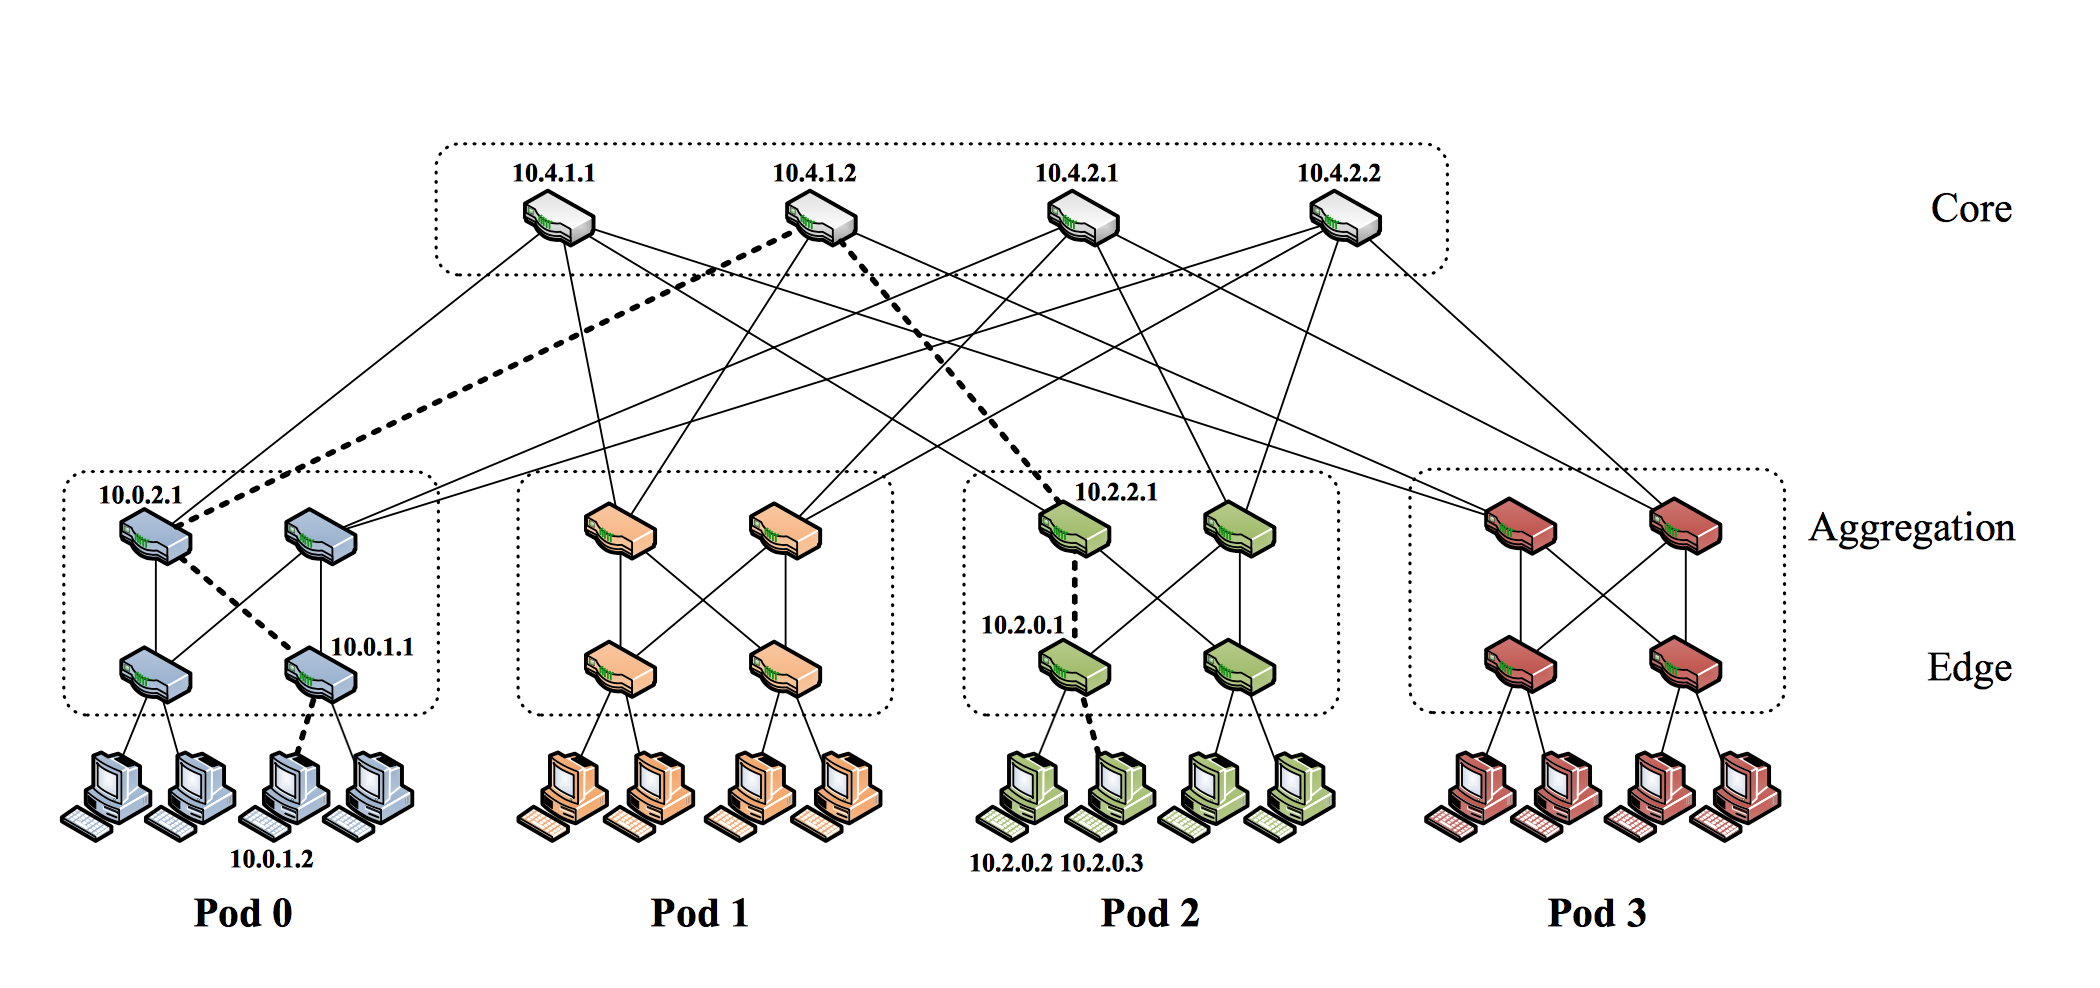
\includegraphics[width=\columnwidth]{figures/fattree.png}
	\caption{Fat Tree Topology}
	\label{fig:fattree}
\end{figure}
Operators can leverage the network structure of topologies
 to reduce the solution space by specifying undesirable path patterns. 
 For example, a path from edge to edge in a fat-tree must not traverse another edge switch.
 This pattern will not drastically reduce the solution space of paths 
 due to the dense interconnect between aggregate and core switches,
 ensuring that synthesis most likely will not fail. 

We introduce tactics\footnote{
	Inspired from use of the term \emph{tactic} in Z3.} 
and labels, abstractions that allow the 
operator to impose a high-level restriction on the paths. 
We use the notion of mapping set of switches to labels to 
have a coarse-grained way for specifying path patterns. This helps
to create search strategies which can be used for majority 
of the packet classes instead of individual switch-level patterns which
lack generality.

 Let $Lb$ be the set of labels and $S$ be the set of switches in the topology. Let $\phi : S \rightarrow Lb$ be the labelling function that maps each switch to a label in $Lb$. One example for $\phi$ in the fat-tree topology in \Cref{fig:fattree} can be that we map all switches in the same level (core, aggregate or edge) to the same label,
therefore leveraging the hierarchical structure of the topology. A path $p$ is a word over the alphabet $S$. 
We define the path-labelling function $\Phi : S^* \rightarrow Lb^*$,  which maps each switch in the path to its corresponding 
 label. 
 For example, given the path $p = e1\ a2\ c3\ a4\ e2$, the path-labeling function function produces $\Phi(p) = eacae$--map each switch to its corresponding label.
 Here, $e$, $a$, and $c$ stand for edge, aggregate, and core respectively.

\subsection{Synthesis with Tactics}
%We use regular expressions and finite automaton to prune the constraints and impose restrictions on the path. The natural way for operators to specify tactics are using \emph{blacklists}, which specify what the path should not be. To express this in a intuitive manner, we use regular expressions on the set of labels to specify blacklists. For example, to blacklist paths from a edge switch to edge switch to not go through another edge switch, we can describe the tactic as $\neg (e .^* e .^* e)$ where the label of all edge switches is $e$. Another tactic is of the form $\neg (e (.)^4 a c .* e)$ which specifies we have a path of length 4, we do not go in the direction towards the core (as to reach the edge, the path would have to then go downwards from the core). 
Tactic are simple regular expressions over the set of labels and are used to blacklist certain path-patterns.
Regular expressions have been previously used in tools like
NetGen~\cite{netgen} to specify the paths for the packet class.
While supporting full regular expressions is possible, it causes a blow-up in the solving time as further
constraints need to be added to the solver to ensure that the path satisfies the regular expression. 
%TODO \loris{is this true?}. % : Cross-check with Aditya. 
Instead, using the notion of switch labels, we use regular expressions to provide high-level path properties as a {\em search strategy} rather than a policy requirement. Instead of specifying how the path must look like, we can use regular expressions on switch labels to specify \emph{blacklists}--i.e.,
what the path must \emph{not} look like. A tactic, for example, can blacklist paths from an edge switch to an edge switch that go through another edge switch. 
%\loris{we need a plot for the full regex thing to compare with Madhu, it would be great to repeat some of their experiments}
 
\subsubsection{Restricted tactic syntax} 
For specifying tactics, we identified a restricted set of regular expressions
 that not only do not require extra constraints to be added,
but actually allow us to reduce the number of constraints. 
This set is defined using the following grammar:
$$\begin{array}{rcl}
R  &  :=  &  \neg (l_{src} .^i C .^* l_{dst}) \\
C  &  :=  &  \varepsilon \mid l_1 \mid l_1 l_2\\
\end{array}$$
where $l_i\in Lb$ and $l_{src}, l_{dst}$ are used to specify the labels of the source switch 
and destination switch, respectively, of the packet classes to which we apply the tactic. 
Since our goal is to black-list paths, we allow regular expressions to be negated at the outer level. 
For example, $\neg (e .^i c .^* e)$ says that the path must not contain an core a switch at the $(i+1)^{th}$ step. 
Similarly, $\neg (e .^i .^* e)$ says that the path connecting two edge switches should have a length $ < i + 1$. 

Let $\pi = sw_0\ldots sw_k$ be a path and 
let its labeling be $\Phi(\pi)= a_0\ldots a_k$.
We say that $\pi$ satisfies a tactic $R$, written $\pi\models R$, if the following
holds:
\begin{compact2itemize}
\item $\pi \models \neg R$ iff $\pi \not\models R$;
\item $\pi \models  l_{src} .^i .^* l_{dst}$ iff $k\geq i+1$, $l_{src}= a_0$, and $l_{dst}= a_k$; 
\item $\pi \models  l_{src} .^i l.^* l_{dst}$ iff $k\geq i+2$, $l_{src}= a_0$, $l_{dst}= a_k$, and $a_{i+1}=l$;
\item $\pi \models  l_{src} .^i l_1 l_2.^* l_{dst}$ iff $k\geq i+3$, $l_{src}= a_0$, $l_{dst}= a_k$, $a_{i+1}=l_1$, and $a_{i+2}=l_2$.
\end{compact2itemize}

Notice that using these constraints we can express more complex forms 
of tactics such as
$\neg (e .^* e .^* e)\equiv \bigwedge \limits_{i=0}^{i=\mu-2} \neg (e .^i e .^* e)$ where $\mu$ is the synthetic limit on path length. 

In \Name, operators can specify conjunctions of tactics which adhere to the restricted syntax and the synthesis algorithm is modified to enforce the tactics. 
Since tactics are path-related restrictions, operators can also apply tactics selectively to the paths for certain packet classes, and also different tactics for different classes. 

\subsubsection{Tactic Synthesis Algorithm}
In our synthesis algorithm, the backward reachability propagation constraints (\Cref{eq:bckprop}) 
construct the path from destination to source. We use tactics to prune these constraints, so that
the path synthesized satisfies the tactic regular expression.  
We describe the tactic synthesis algorithm
for a path $\pi = sw_0 \ldots sw_k$ and labelling $\Phi(\pi) = a_0 \ldots a_k$. 
%In the first
%two cases, we remove some of the reachability constraints by adding negated unit clauses, 
%while we modify these constraints for the next two cases.
%To incorporate tactics in the path for packet class $pc$, we need to modify these constraints. For a path $\pi = sw_0 \ldots sw_k$ and labelling $\Phi(\pi) = a_0 \ldots a_k$, we describe the modifications of the constraints for each type of tactic.
%\loris{this part needs revision. Every time you say we remove constraints, but it actually looks like you are adding extra constraints
%of the form not(..)}

For a tactic of the form $\neg (l_{src} .^i .^* l_{dst})$ which restricts the path to a length $ < i + 1$ we have: 
\begin{equation}
	\pi \models \neg (l_{src} .^i .^* l_{dst}) \Leftrightarrow \forall sw,k \geq i + 1. (sw,pc,k) \notin Reach
\end{equation}
Thus, we can remove the reachability constraints  of \Cref{eq:bckprop} 
for all the tuples $(sw,pc,k) \notin Reach$
as they cannot contribute to any path satisfying the tactic.  

Similarly, we can remove constraints for tactics
of the form $\neg (l_{src}  .^i l .^* l_{dst})$ :
\begin{multline} \label{eq:t1}
\pi \models \neg (l_{src} .^i l .^* l_{dst}) \Leftrightarrow \\ \forall sw.~ \phi(sw) = l ~\wedge~ sw \not= dst \implies  (sw, pc, i + 1) \notin Reach
\end{multline}
The tactic ensures that a switch with label $l$ cannot be reached in $i+1$
steps, except if $l = l_{dst}$. In that case,
only the destination switch with label $l$ can be reached in $i+1$ steps as 
the path with labelling $l_{src}.^i l_{dst}$ satisfies the tactic. If $l \not= l_{dst}$, then
all switches with label $l$ cannot be reached in $i+1$. For all tuples
$(sw, pc, i+1) \notin Reach$, we can remove the reachability constraints of \Cref{eq:bckprop}.
\newline
For tactics of the form $\neg (l_{src}  .^i l_1 l_2 .^* l_{dst})$ : 
\begin{multline} \label{eq:t3}
\pi \models \neg (l_{src} .^i l_1 l_2 .^* l_{dst}) \Leftrightarrow \\ 
\forall n_1, n_2.~\phi(n_1) = l_1~\wedge~ \phi(n_2) = l_2 ~\wedge~ n_2 \not=dst  \implies \\ 
\neg (Reach(n_1, pc, i + 1) \wedge Fwd(n_1, n_2, pc))
\end{multline}
This tactic ensures that a switch with label $l_1$ at $i+1$ in the path
will not forward the packet to a switch with label $l_2$ (unless $n_2$ is the destination). 
To enforce this, we modify the \Cref{eq:bckprop} and remove all $l_1\rightarrow l_2$
edges at position $i+1$ in the path for which $l_2$ is different from the destination.  

%-> if a path is solution of modified constraint it satisfies regex
%<- if a path is solution of original constraints and satisfies regex, then it's a possible solution of modified constraints.

%TODO
\kausik{Write about the path and unmodified constraints, basic facts}
\begin{theorem}
	If the path for a packet class is a solution of the modified constraints, 
	then it satisfies the tactic regular expression.
\end{theorem}
\begin{proof}
Let us prove this theorem by contradiction for each tactic type. \newline
\textbf{Type 1}: $\neg (l_{src} .^i .^* l_{dst})$ \newline
Let us assume that $\pi \models l_{src} .^i .^* l_{dst}$. \\
Thus, $\pi = src\ sw_1 \ldots sw_i \ldots dst$. \\
Therefore,  $(dst, pc, k_{dst}) \in Reach, k_{dst} \geq i + 1$. \\
However,
The modified constraints for this type of tactic are $ \forall sw,k \geq i + 1. (sw,pc,k) \notin Reach$,
which is a contradiction, as $\exists sw, k \geq i + 1. (sw,pc,k) \in Reach$. Hence, our assumption is incorrect. 
\newline \newline
\textbf{Type 2}: $\neg (l_{src} .^i \ l \ .^* l_{dst})$ \newline
Let us assume that $\pi \models l_{src} .^i \ l \ .^* l_{dst}$. \\
Thus, $\pi = src\ sw_1 \ldots sw_i \ sw_{i+1} \ldots dst$ such that $\phi(sw_{i+1}) = l$. Also $sw_{i+1} \not=dst$ (dst has to be the last switch in $\pi$)\\
Therefore,  $(sw_{i+1}, pc, i+1) \in Reach$. \\
However,
The modified constraints for this type of tactic are $\forall sw.~ \phi(sw) = l ~\wedge~ sw \not= dst \implies  (sw, pc, i + 1) \notin Reach$,
which is a contradiction, as $\exists sw. ~ \phi(sw) = l ~\wedge~ sw \not= dst \wedge (sw,pc,i+1) \in Reach$. Hence, our assumption is incorrect. 
 \newline \newline
\textbf{Type 3}: $\neg (l_{src} .^i \ l_1 \ l_2 \ .^* l_{dst})$ \newline
Let us assume that $\pi \models l_{src} .^i \ l_1 \ l_2 \ .^* l_{dst}$. \\
Thus, $\pi = src\ sw_1 \ldots sw_i \ sw_{i+1} \ sw_{i+2} \ldots dst$ such that $\phi(sw_{i+1}) = l_1, \phi(sw_{i+2}) = l_2$. Also $sw_{i+2} \not=dst$ (dst has to be the last switch in $\pi$)\\
Therefore,  $(sw_{i+1}, pc, i+1) \in Reach \wedge (sw_{i+1}, sw_{i+2}, pc) \in Fwd$. \\
However,
The modified constraints for this type of tactic are 
$\forall n_1, n_2.~\phi(n_1) = l_1~\wedge~ \phi(n_2) = l_2 ~\wedge~ n_2 \not=dst  \implies \\ 
\neg (Reach(n_1, pc, i + 1) \wedge Fwd(n_1, n_2, pc))$
which is a contradiction, as $\exists n_1. n_2. ~\phi(n_1) = l_1~\wedge~ \phi(n_2) = l_2 ~\wedge~ n_2 \not=dst \wedge Reach(n_1, pc, i + 1) \wedge Fwd(n_1, n_2, pc)$. Hence, our assumption is incorrect. 
 
\end{proof}


The intuition behind the restricted tactic syntax comes from the structure of the backward reachability propagation 
constraints which construct the path for a packet class. Each constraint says that if a switch is reachable in $k$ steps in a path,
 there must a neighbour switch in the path reachable at $k-1$ steps. We design the restricted tactic syntax based
  on this, providing restrictions on the lengths of the path using $\neg (l_1 .^i .^* l_2)$, or specifying if we cannot 
  reach certain switches at specific positions in the path using  $\neg (l_1 .^i c .^* l_2)$. or specifying local 
  constraints on neighbours using $\neg (l_1  .^i c_1 c_2 .^* l_2)$.  
  
  Conversely, the structure of backward reachability propagation constraints 
  prevents us from being able to specify unrestricted regular expressions. Supporting them
  requires additional constraints to our algorithm which leads to increased synthesis times. 
  Take the following regular expression for example, $\neg(e .^i a c a .*e)$. To enforce
  these tactics, we need to have constraints which prevent the path reaching a aggregate switch in $i+3$
  steps when the path traverses an aggregate and core switch at $i+1$ and $i+2$ steps
  respectively. This cannot be specified by modifying the backward reachability propagation 
  constraints in its current form, 
  because the constraints for reachability for a switch in $i + 3$ steps only depends on 
  the constraints for reachability in $i+2$ steps. Thus, we only support a restricted tactic syntax.   

Incorporating tactics in the synthesis is sound and yield a correct path satisfying all policies.
 However, since tactics artificially reduce the search space, the synthesis algorithm with tactics is incomplete. 
 In practice, tactics can be used to specify restrictions which would be reasonably complete, 
 and speed up the synthesis, especially in datacenter topologies which are hierarchical 
 and can be used to specify interesting tactics. Some examples are : edge-edge path must not
 traverse another edge, and valley-free routing ($eacae$). We have provided a framework for the
 development of new tactics, and we envision entities providing network
 management as a service to develop a \emph{repository} of tactics for various network topologies 
 (much like Z3's tactics), which can be used by network operators without writing tactics of their own. 
%\loris{For that restricted set of regexes the algorithm is trivial you should write the first pass. 
%See the simplified syntax.
%I'll help you with the proof but essentially you have to show that
%if a path $sw_1\ldots sw_k$ satisfies the tactic regex then it is removed (i.e. all constraints necessary
%for it to be encoded have been removed).
%Other direction: if a path was in the original set of constraints and did not 
%satisfy the tactic it has not been removed (also pretty easy)
%}
%\kausik{I think the tactics are quite intuitive to not need a proof of correctness. Do you think we need to explain how we came upon the restricted syntax?
%}
%\loris{No proof is fine. Some intuition would help. Give an example of one that locality can't handle.}

%\subsection{Label Pruning}
%Tactics are an intuitive way to express path properties leveraging the network structure using regular expressions. However, not every permutation of the label alphabet is a valid path in the topology, for example $eaae$ as the aggregate switches are only connected to edge or core switches. Under closer inspection, for a path from an edge switch to another edge switch, we can see that aggregate switches can only occur at odd path length. We describe a label automaton and the algorithm to prune constraints using switch label adjacencies. 
%
%To pruning the constraints using network labels, we construct a label automaton for the topology. The label automaton $A^L$ is an automaton which accepts all words over the alphabet $Lb$ which are a labelling of a valid path in the topology in the topology and rejects all other words. The label automaton has state for each label and transitions for those labels which are connected to that label. We construct the label automaton for the fat-tree topology(\cref{fig:fattree}) in \cref{fig:labelauto}.  
%
%\begin{figure}[h!]
%	\centering
%	\begin{tikzpicture}[shorten >=1pt,node distance=2cm,on grid,auto] 
%	\node[state,initial] (q_0)   {$q_0$}; 
%	\node[state,accepting] (q_a) [right=of q_0] {$q_a$}; 
%	\node[state, accepting] (q_e) [above=of q_a] {$q_e$};
%	\node[state,accepting] (q_c) [below=of q_a] {$q_c$}; 
%	\path[->] 
%	(q_0) edge  node {e} (q_e)
%	edge node {a} (q_a)
%	edge node {c} (q_c)
%	(q_e) edge [bend right=30]  node {a} (q_a)
%	(q_a) edge [bend right=30] node {e} (q_e)
%	edge [bend right=30] node {c} (q_c)
%	(q_c)[bend right=30] edge node {a} (q_a);
%	\end{tikzpicture}
%	\caption{Label automaton $A^L$ for fat-tree topology}
%	\label{fig:labelauto}
%\end{figure}
%For a path starting from an edge switch,  
%using a dynamic programming approach, we build sets $\Gamma(k)$ which is the set of all words starting with $e$ and of length $k$ accepted by the label automaton $A^L$ : $w \in \Gamma(k) \Leftrightarrow w \in L(A^L) \wedge |w| = k$. The algorithm computes $\Gamma(k-1)$, and then the last character of each word can be used to find the state the automaton is in(the automaton reaches the state after reading a particular label), and make a valid transition from that state to construct a word of size $k$ to compute  $\Gamma(k)$. 
%
%Let us define $\Delta(k) := Lb \setminus \{l \ | w \in \Gamma(k) \wedge w[k] = l\}$ to the set of labels which cannot be reached by a path of length $k - 1$ (the length of the label word is one more than length of the path) from an edge switch. For example, in the fat-tree topology in \cref{fig:fattree}:
%\[
%\Delta(1) = \{c, e\} \ \ \ \Delta(2) = \{a\} \ \ \ \Delta(3) = \{c,e\}
%\]
%For each $k \leq \mu$, we can add the following constraints for packet classes which have traverse from a edge-to-edge switch to prune the backward reachability propagation constraints \cref{eq:bckprop}: 
%\begin{equation}
%	\forall sw. \phi(sw) \in \Delta(k) \implies (sw, pc, k -1) \notin Reach
%\end{equation}
%The label automaton pruning is sound and complete because we are using the network structure and network labels to prune certain constraints which cannot be valid, without imposing any restrictions on the path. 
